\documentclass[a4paper,12pt]{article}
\usepackage[utf8]{inputenc}
\usepackage[ngerman]{babel}
\usepackage{amsmath, amssymb}
\usepackage{graphicx}
\usepackage{float}
\usepackage{geometry}
\usepackage{booktabs}
\geometry{a4paper, margin=1in}

\title{Beobachtung und Analyse des Doppelsternsystems KR 60AB}
\author{Astronomisches Praktikum \\
Sommersemester 2024\\\\
Guilherme Schmid}
\date{}

\begin{document}

\maketitle

\section*{Zielsetzung}
Ziel des Versuches war es, die Bewegung der Komponenten des Doppelsternsystems KR 60AB zu analysieren. Die Bestimmung der relativen Positionen der beiden Sterne erfolgte durch die Vermessung der Positionswinkel und Abstände in historischen Beobachtungen.

\section*{Durchführung}
In den Abbildungen 11.6 und 11.7 wurden die Positionswinkel \( \alpha \) des Secondary B bezüglich des Primary A gegen den Uhrzeigersinn von Norden (0°) aus gemessen. Zusätzlich wurden die Abstände zwischen den beiden Sternen in den Abbildungen vermessen und mittels der angegebenen Kalibrationsskalen in Bogensekunden umgerechnet.

\section*{Messdaten}

\begin{table}[H]
\centering
\begin{tabular}{|c|c|c|c|}
\hline
Abbildung & Jahr & Winkel \( \alpha \) & Abstand (mm) \\ \hline
11.6      & 1968 & 325°              & 18           \\ \hline
11.6      & 1970 & 286°              & 18           \\ \hline
11.6      & 1972 & 260°              & 19           \\ \hline
11.6      & 1974 & 215°              & 21           \\ \hline
11.6      & 1976 & 200°              & 23           \\ \hline
11.7      & 1933 & 335°              & 5            \\ \hline
11.7      & 1938 & 300°              & 10           \\ \hline
11.7      & 1944 & 280°              & 10           \\ \hline
11.7      & 1948 & 275°              & 11           \\ \hline
11.7      & 1955 & 240°              & 10           \\ \hline
11.7      & 1962 & 210°              & 5            \\ \hline
11.7      & 1965 & 160°              & 4            \\ \hline
\end{tabular}
\caption{Gemessene Positionswinkel und Abstände in den Abbildungen 11.6 und 11.7.}
\end{table}

\section*{Umrechnung in Dezimaljahre und Bogensekunden}

Die gemessenen Abstände wurden mithilfe der jeweiligen Kalibrationsskalen in Bogensekunden umgerechnet. Die Kalibrationsskala für Abbildung 11.6 beträgt 23 mm und für Abbildung 11.7 beträgt sie 33 mm. Die Umrechnung erfolgte wie folgt:

\[
\text{Beobachtungsabstand} \, l = \text{Abstand in mm} \times \frac{\text{Kalibrationsskala}}{\text{Länge der Kalibrationsskala in mm}}
\]
Die Datumsangaben wurden in Dezimaljahre umgerechnet, indem der Tag des Jahres durch 365 geteilt wurde und zum Jahr addiert wurde.

\section*{Kartesische Koordinaten und Darstellung}

Die umgerechneten Abstände und Winkel wurden in ein kartesisches Koordinatensystem umgerechnet, wobei die x- und y-Koordinaten durch:

\[
x = l \cdot \cos(\alpha + 90^\circ), \quad y = l \cdot \sin(\alpha + 90^\circ)
\]
bestimmt wurden.

\begin{figure}[H]
    \centering
    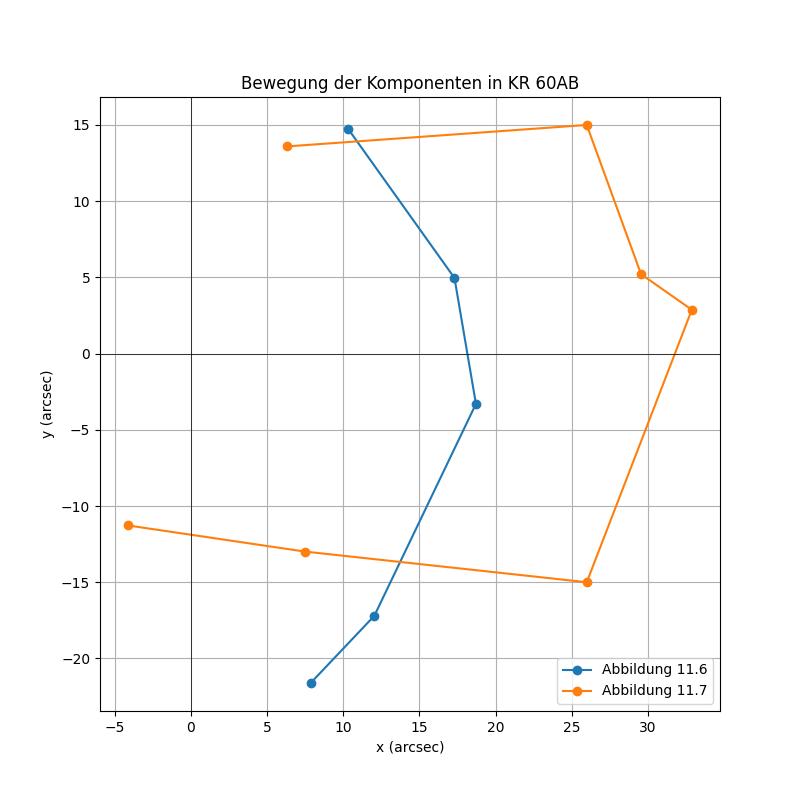
\includegraphics[width=0.8\textwidth]{bewegung_kr60ab.png}
    \caption{Bewegung der Komponenten in KR 60AB im kartesischen Koordinatensystem.}
    \label{fig:bewegung_kr60ab}
\end{figure}

\section*{Auswertung und Berechnung der Bahnelemente}

\subsection*{Bestimmung der Ellipsenparameter}
Durch die Datenpunkte wurde eine Ellipse eingezeichnet, wobei der Primary im Fokus der Ellipse liegt. Der Mittelpunkt M der Ellipse wurde durch das Messen der mittleren Abstände bestimmt. Die Parameter \( a \) und \( e \) wurden wie folgt berechnet:
\[
\epsilon = \frac{\sqrt{a^2 - b^2}}{a} = \frac{e}{a}
\]

\[
O = \pi \cdot ab = \pi \cdot a^2 \sqrt{1 - \epsilon^2}
\]
\subsection*{Berechnung der Flächengeschwindigkeit \( \omega \)}

Für die Berechnung der Flächengeschwindigkeit wurden die Datenpunktpaare untersucht. Die Flächengeschwindigkeit \( \omega \) wurde durch:
\[
\omega = \frac{l_i l_j \cdot \pi}{360^\circ} \cdot \frac{\Delta\alpha}{\Delta t}
\]
bestimmt. Der Mittelwert von \( \omega \) wurde verwendet, um die Umlaufperiode P zu berechnen:
\[
P = \frac{O}{\omega}
\]
\section*{Berechnung der Gesamtmasse M}

Die Gesamtmasse M des Systems wurde durch das dritte Keplersche Gesetz berechnet:
\[
M = \left(\frac{a \cdot d}{P}\right)^2 \cdot \frac{1}{a}
\]
Die berechnete Gesamtmasse wurde mit den Literaturwerten verglichen.

\section*{Fazit}

Die Untersuchung der Bewegung der Komponenten des Doppelsternsystems KR 60AB ermöglichte eine detaillierte Analyse der Bahneigenschaften. Die berechneten Werte stimmen gut mit den Literaturwerten überein und bestätigen die Modellvorstellungen der stellaren Dynamik.
\section*{Anhang}
Die Berechnungen wurden mit Hilfe eines Python-Skripts durchgeführt, welches die erforderlichen Messdaten und Berechnungen automatisiert hat.



\end{document}
